\chapter{Interpreting a Logistic Regression Model \label{chapter:logreg}}

This chapter is similar to Chapter~\ref{chapter:linreg} but focuses on logistic regression models. We first encountered these models as examples of classification algorithms in Chapter~\ref{chapter:classification}. Because of their popularity in the clinical domain, it's important to understand how these models are fit and how to interpret the summary output produced by software. 

%%%%%%%%%%%%%%%%%%%%%%%%%%%%%%%%%%%%%%%%%%%%%%%%%%%%%%%%%%%%%%%%%%%%%%%%%%%%%%%%

\section{ER Readmissions Example from Chapter~\ref{chapter:classification}}

In Chapter~\ref{chapter:classification}, we saw an example where information about two predictors -- a disease severity score ($x_1$) and a social determinants score ($x_2$) -- was used to predict a binary outcome: whether a patient would be readmitted to the ER within 30 days of discharge. We tried three different supervised learning algorithms, one of which was a \textbf{logistic regression} model (Section~\ref{ssect:logreg}). The output from that model is repeated below.

\begin{center}
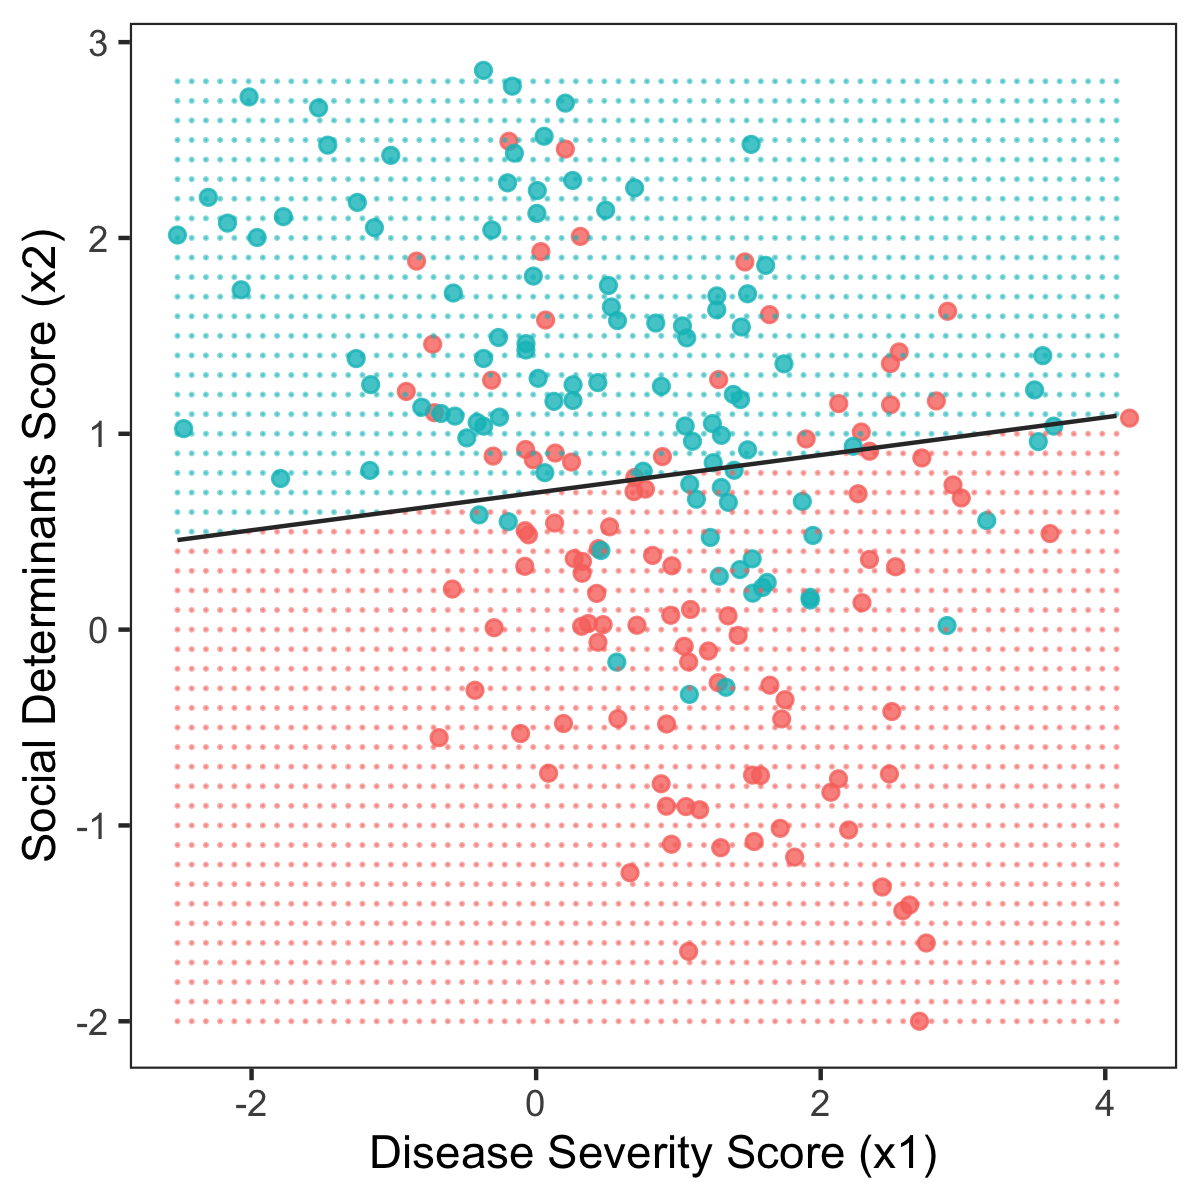
\includegraphics[width=0.35\textwidth]{img/esl-logistic.png}
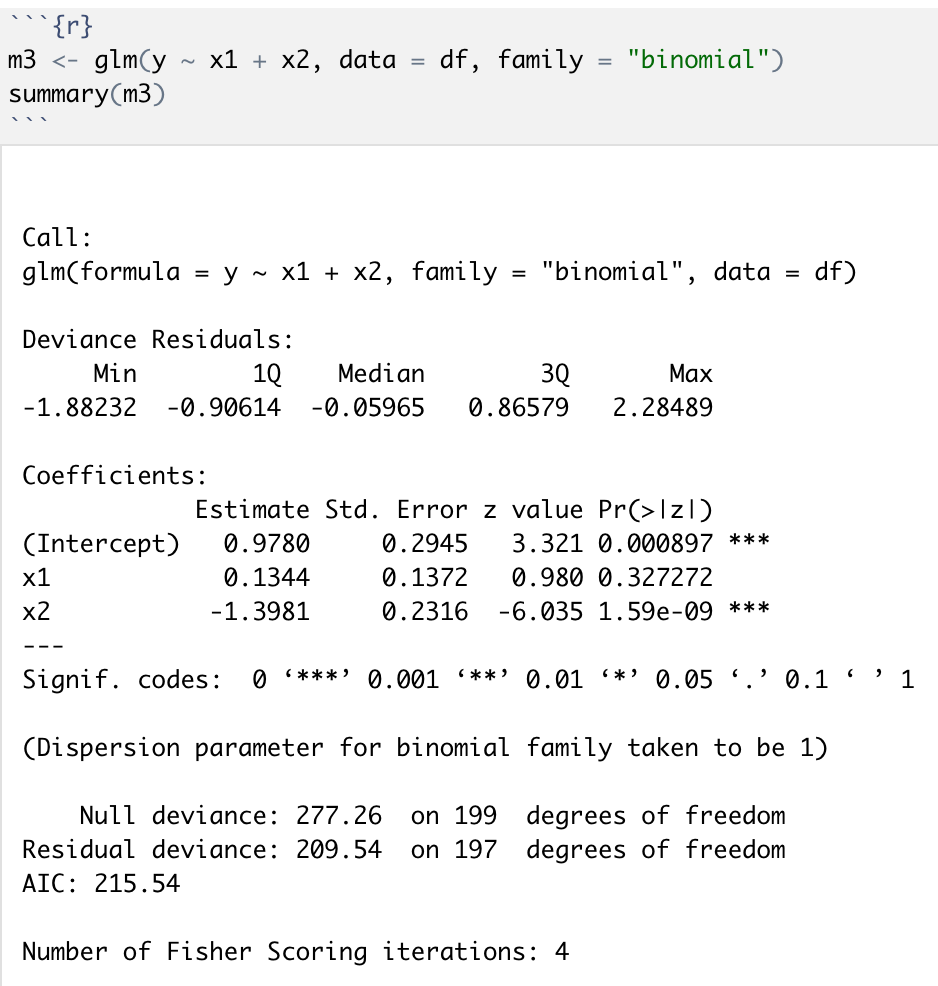
\includegraphics[width=0.64\textwidth]{img/glm-binomial-example.png}
\end{center}

%%%%%%%%%%%%%%%%%%%%%%%%%%%%%%%%%%%%%%%%%%%%%%%%%%%%%%%%%%%%%%%%%%%%%%%%%%%%%%%%

\section{Example: Low Birthweight Dataset}

The goal of this study was to identify risk factors associated with giving birth to a low birth weight baby (a baby weighing less than 2500 grams). Infant mortality rates and birth defect rates are very high for low birth weight babies. A woman's behavior during pregnancy (including diet, smoking habits, and receiving prenatal care) can greatly alter the chances of carrying the baby to term and, consequently, of delivering a baby of normal birth weight.

Data were collected on 189 women, 59 of which had low birth weight babies and 130 of which had normal birth weight babies.

\begin{center}
\texttt{ \small
\begin{tabular}{ll}
\toprule
LOW & Low birth weight (0 = birth weight $\geq$ 2500 g;\\
& 1 = birth weight $< 2500$ g) \\
AGE & Age of mother in years \\
LWT & Mother's weight in pounds at last menstrual period \\
RACE & Race (1 = white, 2 = black, 3 = other) \\
SMOKE & Smoking status during pregnancy (1 = yes, 0 = no) \\
PTL & History of premature labor (0 = none, 1 = one, etc.) \\
HT & History of hypertension (0 = no, 1 = yes) \\
UI & Presence of uterine irritability (0 = no, 1 = yes) \\
FTV & Number of physician visits during the first trimester \\
BWT & Birth weight in grams \\
\bottomrule
\end{tabular}
}
\end{center}
SOURCE: Hosmer and Lemeshow (2000) \emph{Applied Logistic Regression: Second Edition}. Data were collected at Baystate Medical Center, Springfield, Massachusetts during 1986. 

We would like to predict \texttt{LOW} based on all of the other covariates except \texttt{BWT}. (Why not use \texttt{BWT}?) The GLM output of this model is:

{\small
\begin{verbatim}
Call:
glm(formula = LOW ~ AGE + LWT + RACE + SMOKE + PTL + HT + UI + 
    FTV, family = "binomial", data = d)

Deviance Residuals: 
    Min       1Q   Median       3Q      Max  
-1.8946  -0.8212  -0.5316   0.9818   2.2125  

Coefficients:
             Estimate Std. Error z value Pr(>|z|)   
(Intercept)  0.480623   1.196888   0.402  0.68801   
AGE         -0.029549   0.037031  -0.798  0.42489   
LWT         -0.015424   0.006919  -2.229  0.02580 * 
RACE2        1.272260   0.527357   2.413  0.01584 * 
RACE3        0.880496   0.440778   1.998  0.04576 * 
SMOKE        0.938846   0.402147   2.335  0.01957 * 
PTL          0.543337   0.345403   1.573  0.11571   
HT           1.863303   0.697533   2.671  0.00756 **
UI           0.767648   0.459318   1.671  0.09467 . 
FTV          0.065302   0.172394   0.379  0.70484   
---
Signif. codes:  0 '***' 0.001 '**' 0.01 '*' 0.05 '.' 0.1 ' ' 1

(Dispersion parameter for binomial family taken to be 1)

    Null deviance: 234.67  on 188  degrees of freedom
Residual deviance: 201.28  on 179  degrees of freedom
AIC: 221.28

Number of Fisher Scoring iterations: 4
\end{verbatim}
}

\begin{question}{}
In this model, is the effect of one predictor (say, \verb|AGE|) impacted by the value(s) of any of the other predictor(s)? How does this differ from the other classification algorithms we've seen (KNN and decision trees)? What are the advantages and disadvantages of this choice? 
\end{question}

\begin{question}{}
Comment on how the variable \texttt{RACE} enters into the model here. Does this make sense in light of what that variable means and how it potentially interacts with the other study variables?
\end{question}

\begin{question}{}
Interpret the values of each of these coefficients. Based on the coefficient values and their standard errors, which predictor(s) do you think have the greatest impact on whether or not a woman has a low birthweight baby? 
\end{question}

